\pdfminorversion=4
\documentclass[aspectratio=169]{beamer}

\mode<presentation>
{
  \usetheme{default}
  \usecolortheme{default}
  \usefonttheme{default}
  \setbeamertemplate{navigation symbols}{}
  \setbeamertemplate{caption}[numbered]
  \setbeamertemplate{footline}[frame number]  % or "page number"
  \setbeamercolor{frametitle}{fg=white}
  \setbeamercolor{footline}{fg=black}
} 

\usepackage[english]{babel}
\usepackage[utf8x]{inputenc}
\usepackage{tikz}
\usepackage{courier}
\usepackage{array}
\usepackage{bold-extra}
\usepackage{minted}
\usepackage[thicklines]{cancel}
\usepackage{fancyvrb}

\xdefinecolor{dianablue}{rgb}{0.18,0.24,0.31}
\xdefinecolor{darkblue}{rgb}{0.1,0.1,0.7}
\xdefinecolor{darkgreen}{rgb}{0,0.5,0}
\xdefinecolor{darkgrey}{rgb}{0.35,0.35,0.35}
\xdefinecolor{darkorange}{rgb}{0.8,0.5,0}
\xdefinecolor{darkred}{rgb}{0.7,0,0}
\definecolor{darkgreen}{rgb}{0,0.6,0}
\definecolor{mauve}{rgb}{0.58,0,0.82}

\title[2018-09-24-dianahep-histbook]{histbook (and histogramming in Python in general)}
\author{Jim Pivarski}
\institute{Princeton University -- DIANA-HEP}
\date{September 24, 2018}

\usetikzlibrary{shapes.callouts}

\begin{document}

\logo{\pgfputat{\pgfxy(0.11, 7.4)}{\pgfbox[right,base]{\tikz{\filldraw[fill=dianablue, draw=none] (0 cm, 0 cm) rectangle (50 cm, 1 cm);}\mbox{\hspace{-8 cm}
\includegraphics[height=1 cm]{princeton-logo-long.png}
\includegraphics[height=1 cm]{diana-hep-logo-long.png}}}}}

\begin{frame}
  \titlepage
\end{frame}

\logo{\pgfputat{\pgfxy(0.11, 7.4)}{\pgfbox[right,base]{\tikz{\filldraw[fill=dianablue, draw=none] (0 cm, 0 cm) rectangle (50 cm, 1 cm);}\mbox{\hspace{-8 cm}
\includegraphics[height=1 cm]{princeton-logo.png}
\includegraphics[height=1 cm]{diana-hep-logo.png}}}}}

% Uncomment these lines for an automatically generated outline.
%\begin{frame}{Outline}
%  \tableofcontents
%\end{frame}

% START START START START START START START START START START START START START

\begin{frame}{Another histogram package?}
\large
\vspace{0.5 cm}
\begin{columns}
\column{1.05\linewidth}
Histograms are easy to implement, and because they're so essential to HEP analysis, it's worth optimizing the design and experimenting with new ones.

\vspace{0.5 cm}
\textcolor{darkblue}{Is there a downside to creating new histogram packages?}

\vspace{0.2 cm}
\begin{center}
\uncover<2->{Interoperability?}
\end{center}

\vspace{0.2 cm}
\uncover<3->{If Alice uses ROOT, Bob uses Yoda, Claire uses AIDA, and Donald uses Numpy, how are they going to collaborate on analysis?}
\end{columns}
\end{frame}

\begin{frame}[fragile]{Interoperability doesn't have to be hard}
\large
\vspace{0.25 cm}
As long as we're talking about a handful of standards, we can synchronize them.

\begin{columns}
\column{0.5\linewidth}
\small
\vspace{-0.5 cm}
\begin{minted}{python}
import uproot
import numpy
f = uproot.recreate("some.root")
f["myhist"] = numpy.histogram(
    numpy.random.normal(0, 1, 10000))


import ROOT
f = ROOT.TFile("some.root")
h = f.Get("myhist")
h.Draw()
\end{minted}
\column{0.4\linewidth}
\hfill 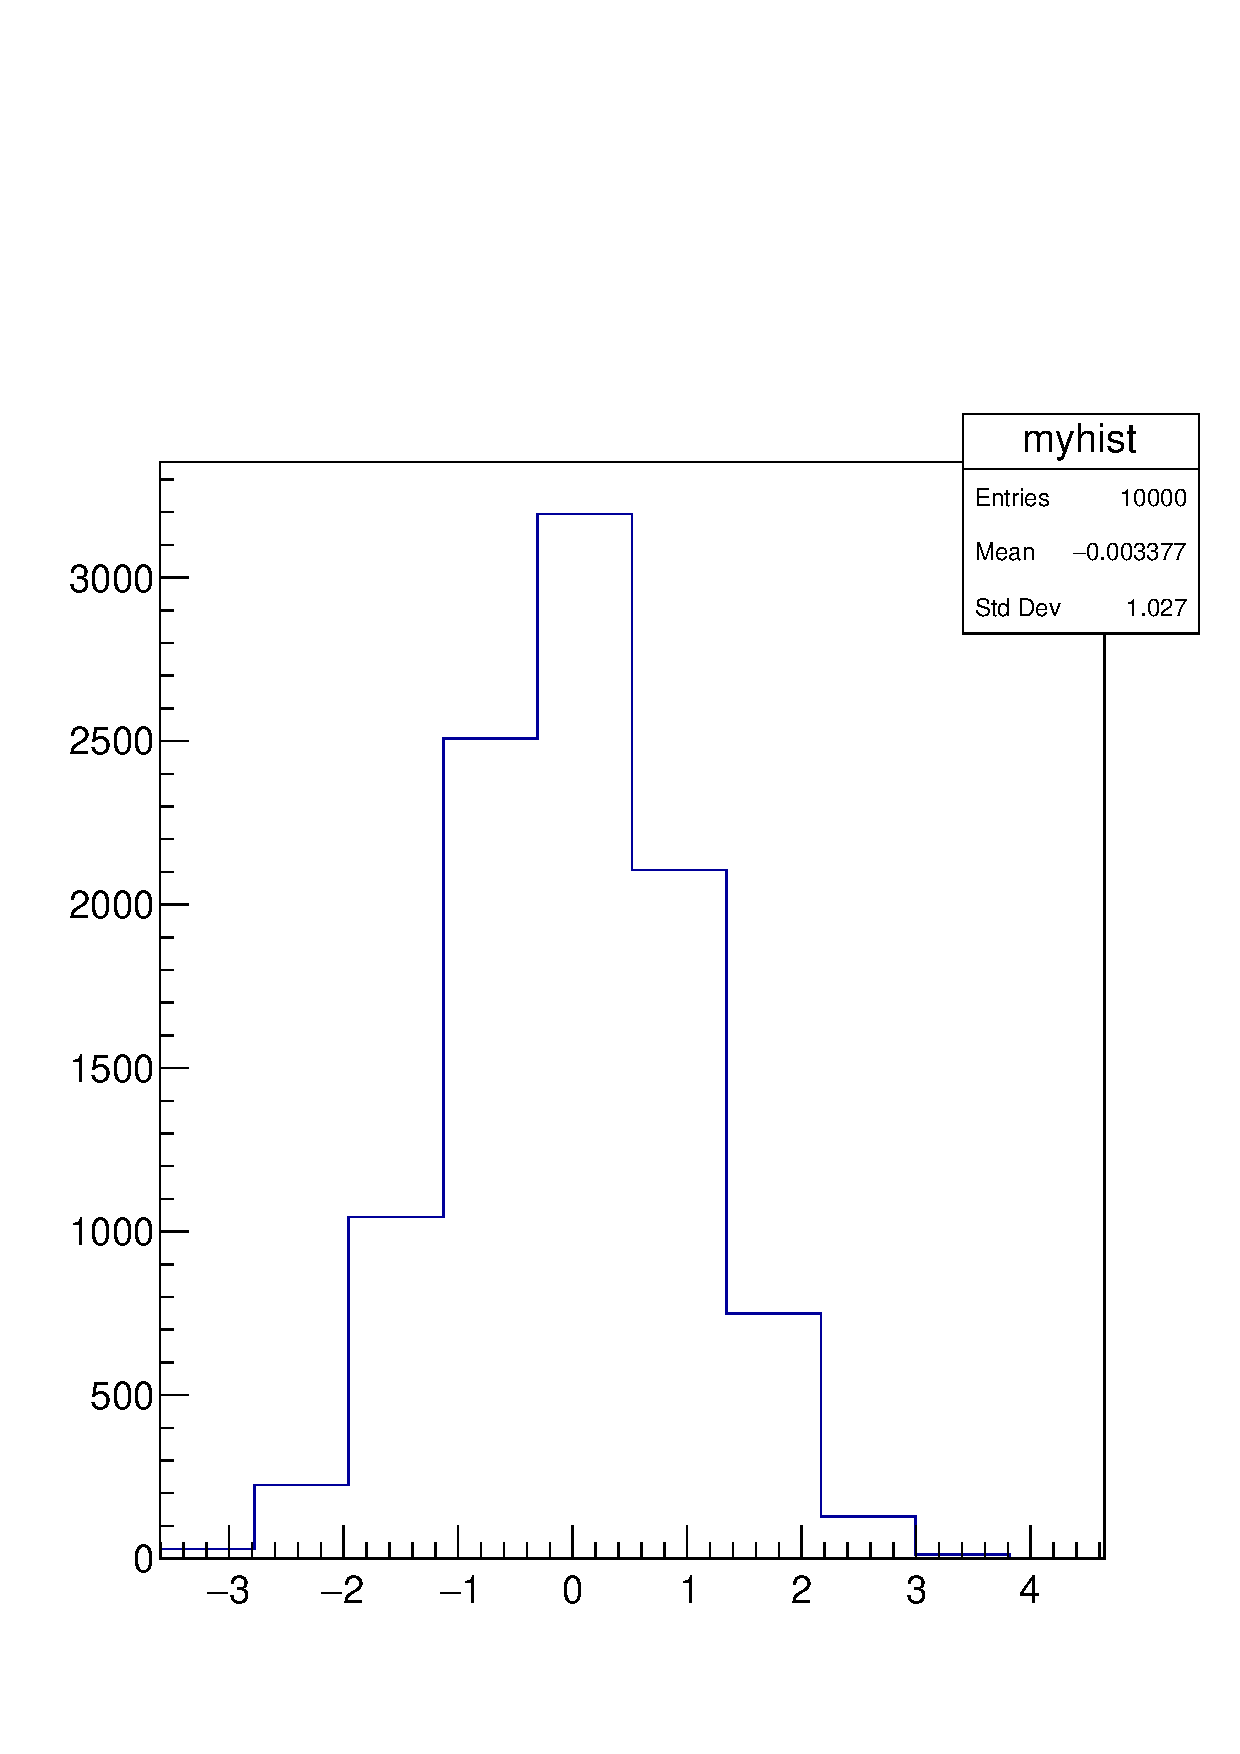
\includegraphics[width=\linewidth]{numpy-to-root.pdf}
\end{columns}

\large
Pratyush Das's histogram-writing feature $+$ a straightforward Numpy translation.
\end{frame}


\end{document}
